The currently supported CAD TestBench model is used to perform a static structural finite element analysis (FEA) on a subset of components from a design space model (see section \ref{sec:designspace}). FEA involves automatically creating an assembly of components of interest, creating a FEA deck consisting of a 3D mesh with load and constraint information, then submitting the deck to a FEA solver to generate results. Results are post-processed via scripts to compute structural metrics. In a test bench model, the user can choose the metric(s) of interest for each component. The currently supported metrics for a structural analysis include:	
\begin{itemize}
\item Factor of Safety
\item Maximum VonMises Stress
\item	Maximum Shear Stress
\item Maximum Bearing Stress
\end{itemize}
Support is currently being added to compute a Quality Rating for the above stress metrics.

\paragraph{Constructing / Syntax}
A CAD TestBench model contains references called TestInjectionPoints that refer to components from a design. The user would include only the components from the design space model for the subsystem that he/she would like to analyze as TestInjectionPoints. Some IFV components are parametric, meaning their CAD models have attributes that need to be specified at runtime during the creation of the assembly for analysis. These attributes appear as CADParameter objects in a component's model in the ValueFlow Aspect and are computed by another interpreter before running FEA. The TopLevelSystemUnderTest object determines the starting point for computing value flow parameters and properties including CADParameters. This typically points to the top most design container in a design space model.

A component surface or a portion of a surface is defined by a group of datum points on the component that form an area that would be constrained or acted upon by a load. The datum points are depicted as ports on the TestInjectionPoint in the test bench model. In the generated 3D mesh, any mesh grid points that fall within the defined area would be constrained or acted upon by a load. To create a surface in the model, the user would connect a Surface object to AnalysisPoint datum ports on a TestInjectionPoint when in Connect Mode in GME. The surface types provided by the modeling language are:  
\begin{itemize} 
\item Circle - Requires three datum points as follows:
		\begin{itemize} 
		\item Point at the center of the circle
		\item Point on the circumference of the circle
		\item Point defining the plane of the circle.  This point would typically (but not necessarily) be on the circumference of the circle; however, it cannot be collinear with the line formed by the first and second points. 
	\end{itemize}
\item Concentric Circles � Two concentric circles defined by three datum points as follows: 
		\begin{itemize} 
		\item Point at the center of the circle
		\item Point on the circumference of the outer circle
		\item Point on the circumference of the inner circle.  Because this point also defines the plane of the circles, it cannot be collinear with the line formed by the first and second points. 
		\end{itemize}
\item Cylinder - Requires 3 datum points as follows: 
		\begin{itemize} 
		\item Point defining the start of the cylinder centerline (i.e. axis)
		\item Point defining the end of the cylinder centerline
		\item Point at a distance from the centerline that equals the cylinder radius.  This point would typically (but not necessarily) be on the cylinder surface.  If it is not on the cylinder surface, it would be offset from the beginning or end of the cylinder.  In any case, the distance between this point and a line defines the radius, where the line is a theoretically infinite line that is coincident with the centerline. 
		\end{itemize}
\item Polygon - Requires at least 3 ordered datum points.  The datum points must be ordered because the order defines the lines segments forming the polygon.  For example, points 1, 2, 3, and 4 would define a polygon with line segments 1-2, 2-3, 3-4, and 4-1.  Noticed that the closing of the polygon by line segment 4-1 is implied.  Repeating 1 at the end (e.g. 1, 2, 3, 4, 1) would be erroneous.      
\item Sphere - Requires 2 datum points as follows:
		\begin{itemize} 
		\item Point at the center of the sphere
		\item Point on the circumference of the sphere
		\end{itemize}
\end{itemize}

 
Loads distort the physical structure thereby creating stress. The CAD TestBench modeling language provides Acceleration (gravity), Force, and Pressure loads. Acceleration is not applied to a single component but to the entire assembly formed by composing TestInjectionPoints. Acceleration is defined by magnitudes in the x, y, z directions. Force load has a Force and a Moment component defined by forces in the x, y, and z directions and moments about the x, y, and z axes. Pressure load is defined by a magnitude value. To apply Force and Pressure loads to a Surface object in the model, the user would connect the Load object to a Surface object when in Connect Mode in GME. Acceleration load is simply placed in the test bench model since it's applied to the composed assembly. A single load object can be connected to multiple Surface objects.

Boundary conditions are used to constrain portions of the model to remain fixed or to be displaced by a prescribed amount. In static structural analysis, boundary conditions are typically used to prevent parts from moving as a rigid body. Boundary conditions provided in the language are: Ball, Displacement, and Pin constraints. Displacement constraint has a Rotation and a Translation component in the x, y, and z direction either as fixed, free or a scalar value. Displacement can only be applied to a Polygonal surface. Pin constraint is defined by a free or fixed AxialRotation and AxialDisplacement attributes and can only be applied to a Cylindrical surface. Ball constraint can only be used on a Spherical surface.  Pin and Ball constraints are currently not supported. To apply constraints to a Surface object in the model, the user would connect a Constraint object to a Surface object when in Connect Mode in GME.

There are three types of Structural Metric objects available in the language: StressMetric, FactorOfSafety, and MaximumDisplacement. The StressMetric has a Type attribute which the user can set to either Mises, Shear, or Bearing. The Type attribute determines which stress types appear in the resulting log and Dashboard XML file after post-processing analysis results. A StressMetric object should be connected to TestInjectionPoint(s) of interest.  The stress metric is only computed for the connected TestInjectionPoint(s).

\begin{figure}[t]
\centering
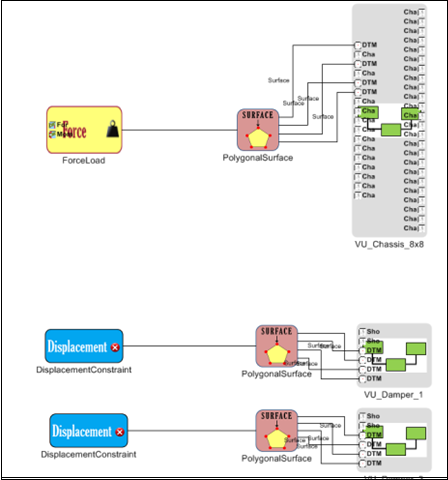
\includegraphics[scale=0.40]{Figures/chassisDamper_cadTB.png}
\caption{Chassis Damper Cad Test Bench.}
\label{fig:chassis_damper}
\end{figure}

Figure \ref{fig:chassis_damper} shows portions of the Chassis Damper CAD TestBench model in the current IFV model. This test bench is used to analyze a single chassis along with eight connecting dampers to compute stress distributions under a set of loads and constraints. There are nine TestInjectionPoints, one for chassis and eight for the eight dampers. There is a single Force load on the chassis with a scalar value in the y direction on the Force component. All eight of the dampers have a displacement constraint with rotation in the y direction set to free and all other attributes set to fixed. Only polygonal surfaces are used for the loads and constraints and they are connected to datums in each component. The connections themselves are annotated with Surface to indicate the location. Similarly, when other types of Surface objects are connected to datum points the connection would be annotated to show the point's location on a Surface object.

\paragraph{Executing}
\begin{figure}[t]
\centering
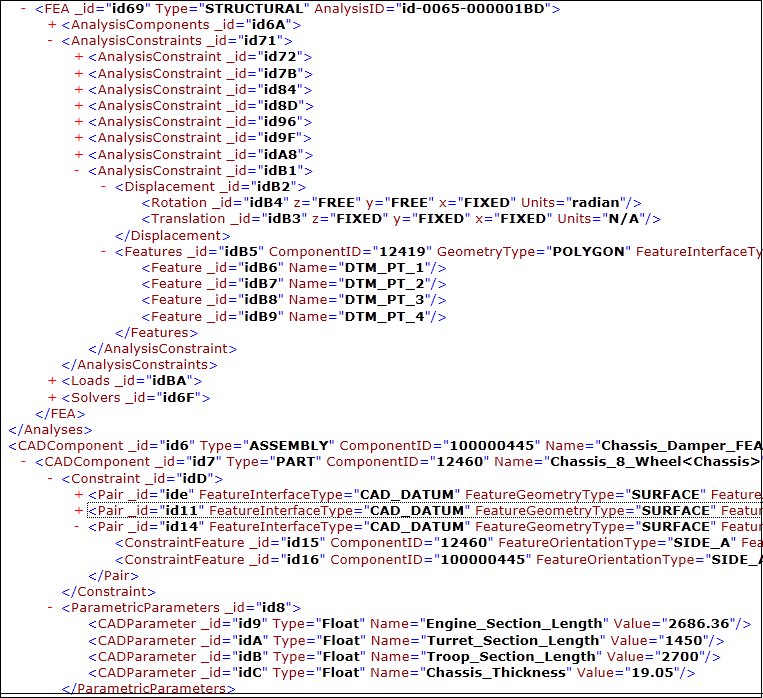
\includegraphics[scale=0.40]{Figures/xmlOut_cadTB.png}
\caption{XML file generated from CyPhy2CAD with assembly information and FEA load and constraints.}
\label{fig:cadTB_xml}
\end{figure}
The CyPhy2CAD interpreter processes a test bench model and produces an XML file containing the assembly definition.  The assembly definition specifies how components are constrained to one another via datums, and it specifies the FEA loads and constraints.  Figure \ref{fig:cadTB_xml} shows the generated XML file. The interpreter requires 2 directories, one for storing the generated files and a second one for the location of Creo part files.

\begin{figure}[t]
\centering
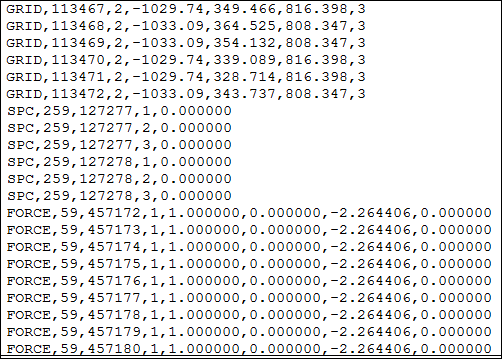
\includegraphics[width=0.5\textwidth]{Figures/inpDeck_cadTB.png}
\caption{XML file generated from CyPhy2CAD with assembly information and FEA load and constraints.}
\label{fig:inpDeck_cadTB}
\end{figure}
A program called CADCreoParametricCreateAssembly is invoked that calls Creo SDK APIs to automatically build a Creo assembly based on the xml file as well as calling Creo's mesher to generate a 3D mesh of the assembly in the form of a Nastran input deck, see figure \ref{fig:inpDeck_cadTB} for a section of the deck. In the figure, GRID keyword is followed by coordinates of grid points in the mesh, SPC keyword corresponds to constraints from the model applied to mesh grid points, and lines with FORCE keyword are Force loads on grid points. A bat file calls a FEA solver passing in the Nastran input deck as the argument. Currently we are using Abaqus from SIMULIA as our solver and are working on supporting more solvers. Abaqus returns several files, but the main one we post-process is a binary data file (*.odb file). The post-processing step involves computing the maximum stresses (VonMises, Shear, and Bearing) and factory of safety based on the maximum stresses and material properties for component(s). PNG files showing stress gradients across component(s) in 7 views (iso, top, bottom, left, right, back, and front), VRML, and 3D Xml files are also generated. 3D XML file contains 3D data that can be opened in a player to view stress gradients and animated deformations. A log file is generated that contains status and error messages as well as metric information for debugging purposes. An XML file conforming to Dashboard schema is generated so that the metrics can be visualized in the Dashboard.

Figure \ref{fig:isogradient} shows the output stress gradient png file in the iso view. Notice that high stress areas are marked by red and low stress area by blue.

\begin{figure}
\centering
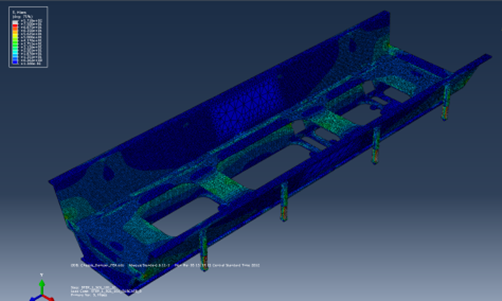
\includegraphics[scale=0.40]{Figures/iso_gradient_cadTB.png}
\caption{ISO view of stress gradient in Chassis.}
\label{fig:isogradient}
\end{figure}